\message{ !name(masters.tex)}\documentclass[]{spie}  %>>> use for US letter paper

\usepackage{graphicx}
\usepackage{subfig}
\usepackage{amsmath}
\usepackage{amssymb}
\usepackage{hyperref}
\usepackage{float}
\usepackage{multirow}

\title{Texture Mapping 3D Models of Indoor Environments with Noisy Camera Poses} 

\author{Peter Cheng
\skiplinehalf
University of California, Berkeley\\
}

\begin{document}

\message{ !name(masters.tex) !offset(890) }
\subsection{Exposure Compensation}
\label{sec:exposureCompensation}

\begin{figure}
  \centering
  \subfloat[][]{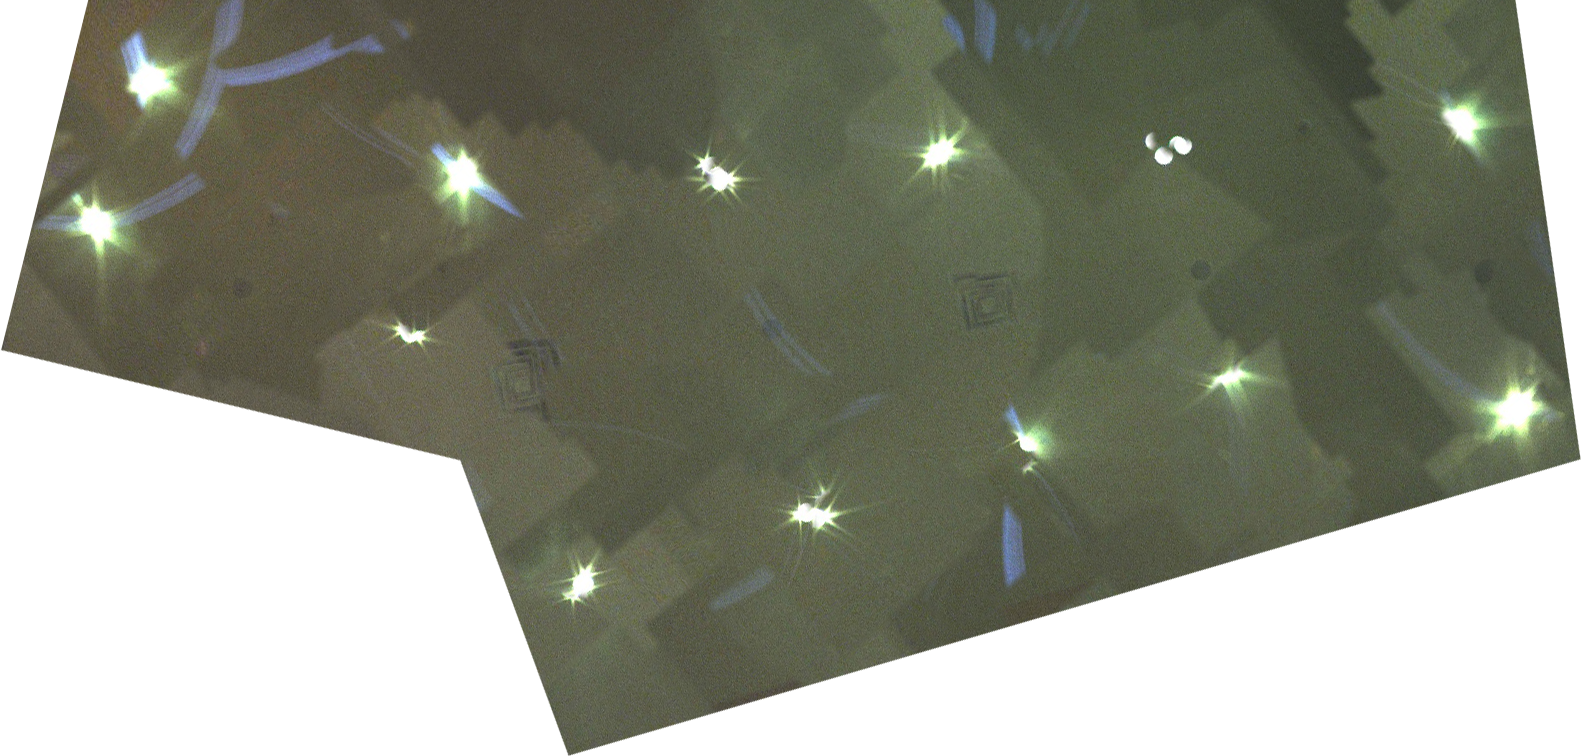
\includegraphics[width=3.3in]{exposureDiff1.png}}
  \subfloat[][]{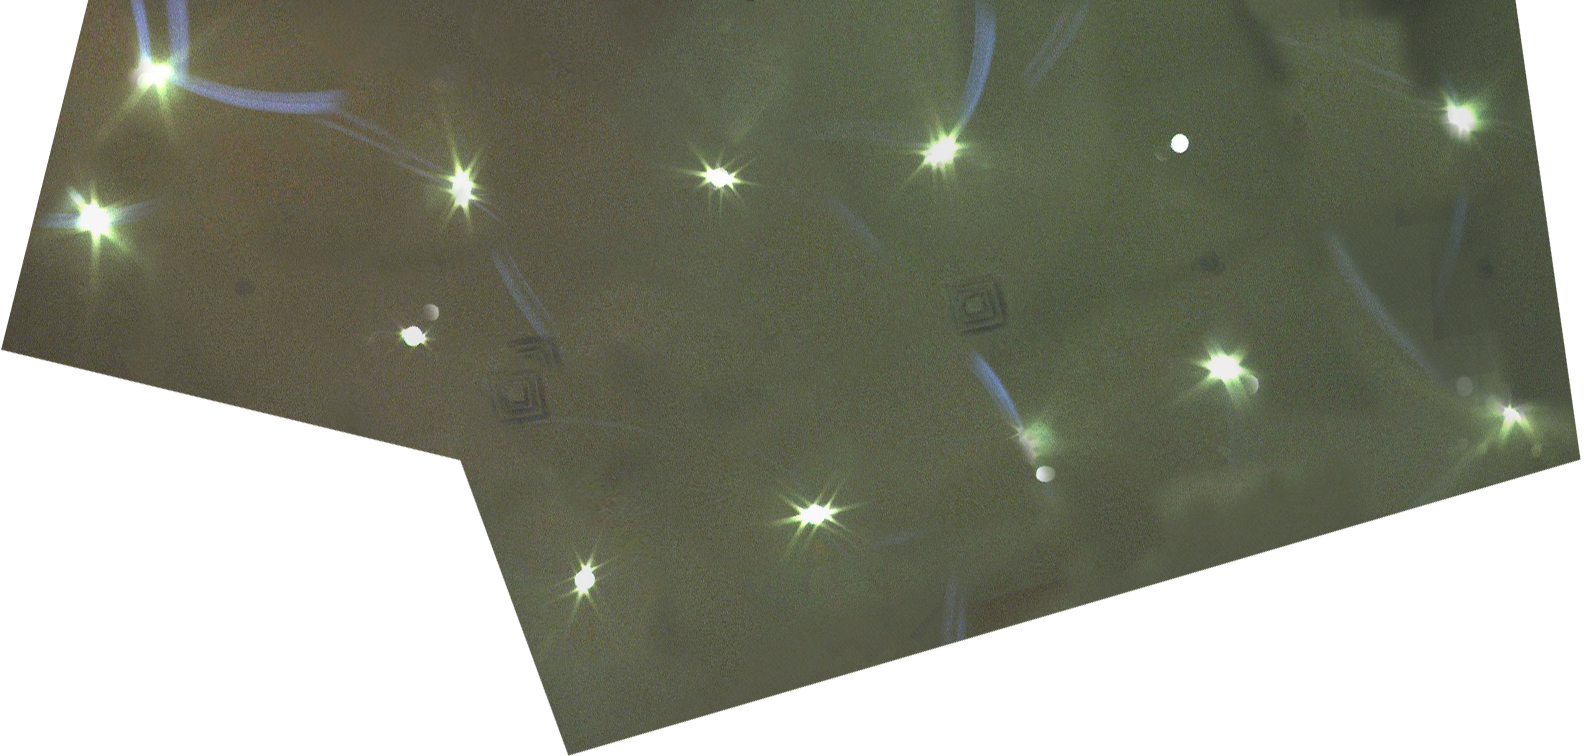
\includegraphics[width=3.3in]{exposureDiff2.png}}
  \caption{(a) A ceiling texture composed of images taken with varying
    exposures, with significant brightness differences. (b) Exposure
    compensation applied to the same set of images from (a) by
    applying computed gains to each image}
  \label{fig:exposureDiff}
\end{figure}


Before blending images together, exposure compensation is applied to
equalize brightness among neighboring images. For the images in this
report, cameras are set to have automatic exposure, which means that
images of the same object may have different brightness levels. While
successful image alignment and blending can reduce sharp seams between
adjacent images, there may still be noticeable brightness gradients
between images, particularly in areas near light sources. This can be
seen in Figure \ref{fig:exposureDiff}(a), where the ceiling texture
has patches of clearly differing brightness, most noticeably around
light sources. To diminish this effect, a gain can be computed and
applied to each image, with the effect of linearly scaling the
brightness of an image. The goal is to compute a gain for each image,
such that the brightness of an area is consistent across image
boundaries.

Similar to the image location adjustment procedure in Section
\ref{sec:robustSIFTFeatureMatching}, exposure compensation can be
neatly formed as a least-squares optimization problem with pair-wise
observations. In this case, observations do not need to be weighted,
and so the formulation is $\textrm{min}_{\vec{\beta}} ||(A \vec{\beta}
- \vec{\gamma})||_2^2 $. An example setup for 3 images, each with 2
overlapping pixels is shown below.
\[
A =
\begin{pmatrix}
  P_{11} & -P_{12} & 0\\
  P_{21} & -P_{12} & 0\\
  0 & P_{32} & -P_{33}\\
  0 & P_{42} & -P_{43}\\
  1 & 1 & 1\\

\end{pmatrix}\quad
\vec{\beta} =
\begin{pmatrix}
  G_1, \\ G_2, \\ G_3
\end{pmatrix}
\vec{\gamma} =
\begin{pmatrix}
  0, \\ 0, \\ 0, \\ 0, \\ 3
\end{pmatrix}
\]

In this problem, $\beta$ is the vector of gains $G_i$ to be solved
for.  The observations, represented by $A$ and $\gamma$, correspond to
equalizing the brightness for each pixel present in two images. For
instance, for pixel $P_x$ which is present in two overlapping images
$I_i$ and $I_j$, the goal is to find gains $G_i$ and $G_j$ such that
$G_iP_{xi} - G_jP_{xj} = 0$, where $P_{xy}$ is the value of pixel
$P_x$ in image $I_y$. Thus, $\gamma$ contains all zeros, while each
row of $A$ contains a $P_i$ value in the $ith$ column and a $-P_j$
value in the $jth$ column, and zeros elsewhere. The number of
observations is thus equal to the number of pixels that occur in two
distinct images.  This problem is not constrained, as it allows all
computed gains to be scaled by any amount. To keep gains at reasonable
values, a final observation is added: $\Sigma G_i = N$, where $N$ is
the number of images. This has the effect of averaging all gains to 1.

The result of computing gains and equalizing exposure can be seen for
the same ceiling location in Figure \ref{fig:exposureDiff}(b). The
effect is clear, as dark/bright patches are no longer present, and the
overall brightness of the image has not changed significantly.

\message{ !name(masters.tex) !offset(1248) }

\end{document} 
